% Created 2015-08-31 Mon 19:32
\documentclass[11pt,oneside]{memoir-article}
\usepackage{calculating-the-uposatha-moondays}
\renewcommand{\docVersion}{v0.4}
\renewcommand{\docUrl}{\href{https://github.com/profound-labs/calculating-the-uposatha-moondays/}{link}}
\hypersetup{ pdfauthor={Gambhiro Bhikkhu}, }
\author{Gambhiro Bhikkhu}
\date{\today}
\title{Calculating the Uposatha Moondays}
\hypersetup{
  pdfkeywords={},
  pdfsubject={},
  pdfcreator={Emacs 25.0.50.1 (Org mode 8.2.10)}}
\begin{document}

\maketitle
\begin{tldr}
\begin{itemize}
\item This is composed as a manual on how to calculate the Full- and New
Moon day \emph{uposathas}, indicating the astronomical cycles that
underlie the method.
\item The method is based on a set of formulas called \emph{suriyayatra},
including additional rules observed in Thailand.
\item Alternate 30 and 29 day lunar months, 12 months make one year. Add
an extra month 7 times in every 19 years, add an extra day 11 times
in every 57 years.
\item Conventions on how to practise this can differ by countries and
groups, resulting in self-consistent but different calendars.
\item The Royal Thai Calendar defies exact prediction with unforeseen
adjustments, the different monastic groups simply adjust the major
moondays in their calendars for concord.
\end{itemize}
\end{tldr}

\begin{quote}
Much appreciation for the answers from the Venerable Ajahns who
endured my questions. Comprehension and consistency was only possible
with their experience and understanding.

Download \href{https://github.com/profound-labs/calculating-the-uposatha-moondays/raw/master/calculating-the-uposatha-moondays.pdf}{this PDF} or a \href{https://github.com/profound-labs/calculating-the-uposatha-moondays/archive/master.zip}{ZIP archive} with references.

Comments, corrections and further information would be greatly
appreciated:

\texttt{Gambhiro Bhikkhu <gambhiro.bhikkhu.85@gmail.com>}

\textbf{Changelog:}

2015-08-31, v0.4
\begin{itemize}
\item tutorial completed
\item year diagram, year planners
\item general review
\end{itemize}
2015-08-04, v0.3
\begin{itemize}
\item Uposatha Calendar Tutorial
\end{itemize}
2014-10-09, v0.2
\begin{itemize}
\item Ven. Hāsapañño:
\begin{itemize}
\item adhikavāra clarified
\item first and last day of a lunar month
\item occurrence of major moondays with the Pāli method
\end{itemize}
\end{itemize}
2014-10-07, v0.1
\begin{itemize}
\item ready for feedback
\end{itemize}
\end{quote}

\clearpage

\chapter{Mahānikāya Uposatha Calendar Tutorial}
\label{sec-1}

This section is a step-by-step guide on how to calculate the uposathas for a
given year.

I recommend printing the following pages to be able to reference them as you follow along:

\begin{itemize}
\item The diagram on p.\pageref{dia-common-adhikamasa-adhikavara} shows the
uposathas in a common-, adhikamāsa- and adhikavāra year.
\item There are A4 format year planners included for 2015 (p.\pageref{year-2015}),
2016 (p.\pageref{year-2016}) and 2017 (p.\pageref{year-2017}). This is a
sequence of an adhikamāsa, adhikavāra and a common year.
\end{itemize}

\section{Collecting information about the year}
\label{sec-1-1}

We need to know the following:

\begin{itemize}
\item the last uposatha of the previous lunar year
\item whether there is an extra lunar month (adhikamāsa),
\item or an extra day (adhikavāra),
\item or neither, and so it is a common year.
\end{itemize}

Find the Full Moon in last year November, this is the last uposatha of the
previous lunar year.

In Thai practice a lunar year can't have both an adhikamāsa and an adhikavāra.

Table \ref{tbl-cycle-adhikamasa} shows a few adhikamāsa years. See if the given
year will have an adhikamāsa.

Table \ref{tbl-cycle-adhikavara} shows a few adhikavāra years. Keep in mind that
this is provisional. Even when a year qualifies for an adhikavāra, the calendar
authorities may choose to add it in a different year.

Now we know that the year is either:

\begin{itemize}
\item a common year,
\item an adhikamāsa year, or
\item an adhikavāra year.
\end{itemize}

Gregorian leap years don't affect the lunar calendar, but it may be useful to
check when planning ahead. Table \ref{tbl-cycle-leap-years} shows a few leap
years.

\section{Common year}
\label{sec-1-2}
\label{common-year}
\subsection{Alternate 30 and 29 day months}
\label{sec-1-2-1}

Counting from the last Full Moon of the previous lunar year (which will be in
November), the first month is 30 days, the second is 29 days:

\begin{center}
\begin{tabular}{lll}
15 days & \GaNewmoon{} New Moon & First uposatha of the Cold Season\\
15 days & \GaFullmoon{} Full Moon & End of first month, 30 days\\
14 days & \GaNewmoon{} New Moon & \\
15 days & \GaFullmoon{} Full Moon & End of second month, 29 days\\
\end{tabular}
\end{center}

A Full Moon is always on the 15th day. Every second New Moon is on the 14th day.

The \GaWaxingmoon{} Waxing- and \GaWaningmoon{} Waning Moons are on the 8th day.

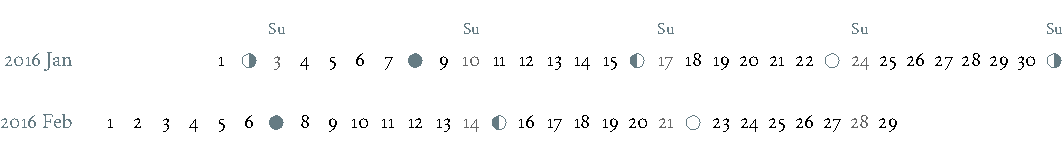
\includegraphics[width=\linewidth]{two-months.pdf}

Keep alternating 30 and 29 day months. One season is four months, one year is
three seasons: Cold-, Hot- and Rainy Season. See Table \ref{tbl-month-names} for
the Pāli names of months and seasons.

\subsection{Marking the Vassa and Major Moondays}
\label{sec-1-2-2}

Mark the months and seasons according to Table \ref{tbl-month-names}.

The key annual events are on the Full Moon of the given lunar months:

\begin{center}
\begin{tabular}{ll}
 & Lunar Month\\
Māgha Pūjā & 3rd\\
Visākha Pūjā & 6th\\
Āsāḷha Pūjā & 8th\\
Pavāraṇā Day & 11th\\
\end{tabular}
\end{center}

Mark the Vassa (Rainy Season Retreat):

\begin{itemize}
\item The first day of the Vassa is the day after Āsāḷha Pūjā
\item The last day of the Vassa is Pavāraṇā Day
\end{itemize}

In a common year, the calendar is finished. 

\section{Adhikamāsa year}
\label{sec-1-3}
\subsection{Marking the Vassa and Major Moondays}
\label{sec-1-3-1}

Adding the extra month has three consequences:

\begin{itemize}
\item the Major Moondays shift to the next Full Moon
\item Gimhāna (Hot Season) has 10 uposathas instead of 8
\item the Vassa starts 30 days later
\end{itemize}

The extra month is a 30 day month. In Thai practice, it is appended to the end
of the Hot Season, after the 8th month (Āsāḷha). The convention is to call this
the `second 8th' or `second Āsāḷha', marked as 8/8.

Āsāḷha Pūjā will be held in the 8/8 2nd Āsāḷha month, after which will be the
first day of the Vassa. The Vassa remains the same length, 8 uposathas.

Āsāḷha Pūjā and Pavāraṇā Day therefore shifted because we added an extra month
to the end of the Hot Season.

From a practical perspective, Māgha Pūjā and Visākha Pūjā are simply moved to
the next month, and are marked in the 4th and 7th month instead of the 3rd and
6th. This is as though it happened in a parallel, separate system, and it
doesn't influence the actual numbering or length of the months.

This has the advantage that there will not be a large gap between Visākha and
Āsāḷha Pūjā (now in the 2nd Āsāḷha). See sec.\ref{marking-the-moondays} for a
further discussion of the logic.

See the diagram on page \pageref{dia-common-adhikamasa-adhikavara} to compare
how the sequence of the uposathas and the major moondays fall in an adhikamāsa
year compared to a common year.

\subsection{Thai and monastic lunar months}
\label{sec-1-3-2}

In addition, there is a monastic and a Thai way of reckoning the beginning and the
end of the lunar months. When looking up information, one needs to find out
which system is being used.

In the monastic lunar months, the Full Moon is on the last day of the month.

In the Thai lunar months, the Full Moon is in the middle of the month, and the
New Moon is on the last day.

\section{Adhikavāra year}
\label{sec-1-4}

The extra day is inserted in the 8th month (Āsāḷha), making the 7th uposatha of
the Hot Season a 15-day uposatha instead of the expected 14-day, and making
Āsāḷha a 30-day month that year.\cite{hasapannyo-zodiac}

In adhikavāra years the Vassa starts one day later.

\begin{center}
\begin{tabular}{rlr}
order & name & days\\
\hline
6 & Visākha & 29\\
7 & Jeṭṭha & 30\\
8 & Āsāḷha & \textbf{30}\\
9 & Savaṇa & 30\\
10 & Bhaddapāda & 29\\
\end{tabular}
\end{center}

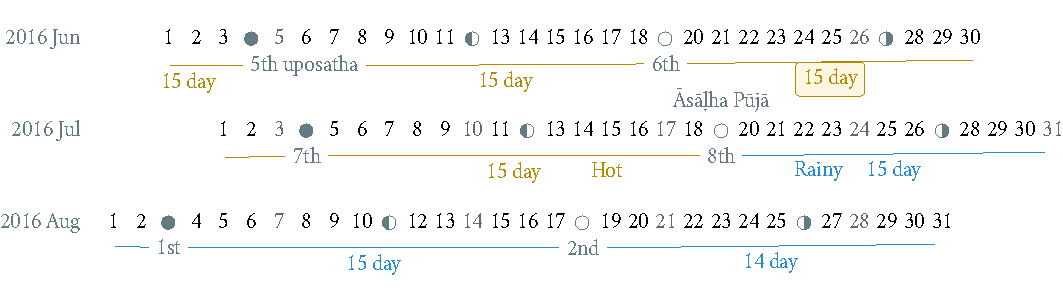
\includegraphics[width=\linewidth]{adding-the-extra-day.pdf}

\clearpage

\chapter{The Mahānikāya Uposatha Calendar Method}
\label{sec-2}
\section{Adding the extra month}
\label{sec-2-1}

The extra month (adhikamāsa) is added 7 times in every 19 year, in a repeating
pattern of 3-3-2 - 3-3-3-2 years. This is a shorthand for the formulas
at \ref{fig-suriyayatra} which generate this pattern. Table
\ref{tbl-cycle-adhikamasa} shows adhikamāsa years for 1985-2039.

In Thai practice, the extra month is a 30 day month inserted after the
8th month (\emph{Āsāḷha}), at the end of the Hot Season. The convention is
to call this the `second 8th' or `second \emph{Āsāḷha}', marked as 8/8.

In adhikamāsa years the Vassa starts 30 days later, after the 2nd
Āsāḷha, on the day after the Full Moon uposatha of 8/8.

\begin{center}
\begin{tabular}{rlr}
order & name & days\\
\hline
8 & Āsāḷha & 29\\
8/8 & 2nd Āsāḷha & 30\\
9 & Savaṇa & 30\\
\end{tabular}
\end{center}

\begin{table}[h]
\caption{\label{tbl-cycle-adhikamasa} Adhikamāsa years}\legend{\Delta m: years since the last adhikamāsa. Nth: place in the 19-year cycle.}
\centering
\begin{tabular}{rrrr}
 &  & $\Delta$ m & Nth\\
\hline
1985 & 2528 & 3 & 3\\
1988 & 2531 & 3 & 6\\
1990 & 2533 & 2 & 8\\
1993 & 2536 & 3 & 11\\
1996 & 2539 & 3 & 14\\
1999 & 2542 & 3 & 17\\
2001 & 2544 & 2 & 19\\
2004 & 2547 & 3 & 3\\
2007 & 2550 & 3 & 6\\
2009 & 2552 & 2 & 8\\
2012 & 2555 & 3 & 11\\
2015 & 2558 & 3 & 14\\
2018 & 2561 & 3 & 17\\
2020 & 2563 & 2 & 19\\
2023 & 2566 & 3 & 3\\
2026 & 2569 & 3 & 6\\
2028 & 2571 & 2 & 8\\
2031 & 2574 & 3 & 11\\
2034 & 2577 & 3 & 14\\
2037 & 2580 & 3 & 17\\
2039 & 2582 & 2 & 19\\
\end{tabular}
\end{table}


\clearpage

\subsection{Marking the Major Moondays}
\label{sec-2-1-1}
\label{marking-the-moondays}

TODO

\section{Adding the extra day}
\label{sec-2-2}
\label{adding-extra-day}

The extra day (adhikavāra) is added 11 times in every 57 year.

Whether a year should have an extra day can be determined with the
conditions at sec.\ref{adhikavara-years}.

In Thai practice a year with an extra month is not allowed to also
have an extra day. If the year should have an extra day, but it
already has an extra month, the extra day is assigned to one of the
flanking years (next or previous, in the case of planning several
years in advance).

In adhikavāra years the Vassa starts one day later.

If the year is going to have an extra day, it is inserted in the 8th month
(Āsāḷha), making the 7th uposatha of the Hot Season a 15-day uposatha instead of
the expected 14-day, and making Āsāḷha a 30-day month that
year.\cite{hasapannyo-zodiac}

\begin{center}
\begin{tabular}{rlr}
order & name & days\\
\hline
6 & Visākha & 29\\
7 & Jeṭṭha & 30\\
8 & Āsāḷha & \textbf{30}\\
9 & Savaṇa & 30\\
10 & Bhaddapāda & 29\\
\end{tabular}
\end{center}

However, this is the most unpredictable variable in the calendars published for
a given year, and the various calendar authorities add the extra day in a
flexible manner, in some of cases adding it in the years according to the
formula but deviating from it in others.


Nonetheless they observe that:

\begin{itemize}
\item the count for 11 times in 57 years is maintained to keep the
calendar at pace
\item the extra day will not be in years that also have an extra month.
\end{itemize}

\begin{table}[h]
\caption{\label{tbl-cycle-adhikavara} Adhikavāra years}\legend{K, A, T for kammacubala, avoman and thaloengsok}
\centering
\begin{tabular}{rrrrr}
Year & CS & K & A & T\\
\hline
1994 & 1356 & 535 & 54 & 6\\
2000 & 1362 & 93 & 627 & 11\\
2005 & 1367 & 658 & 656 & 7\\
2009 & 1371 & 630 & 119 & 22\\
2014 & 1376 & 395 & 137 & 17\\
2016 & 1378 & 781 & 566 & 9\\
2020 & 1382 & 753 & 29 & 24\\
2025 & 1387 & 518 & 47 & 19\\
\end{tabular}
\end{table}

\clearpage

\section{Major Moondays}
\label{sec-2-3}
\label{major-moondays}

Buddhist communities observe the key annual events on and around the Full Moon
days of the 3rd, 6th, 8th and 11th lunar months, see Table \ref{tbl-major-events}.

\begin{table}[h]
\caption{\label{tbl-major-events} Major Events in a Common Year}
\centering
\begin{tabular}{ll}
Event & Time\\
\hline
Māgha Pūjā & 3rd Full Moon\\
Visākha Pūjā & 6th Full Moon\\
Āsāḷha Pūjā & 8th Full Moon\\
First Day of Vassa & the day after Āsāḷha\\
Pavāraṇā Day & 11th Full Moon\\
Last Day of Vassa & Pavāraṇā Day\\
\end{tabular}
\end{table}

Also see sec.\ref{lunar-month-first-last} on \emph{Thai} lunar months.

\clearpage

\chapter{The Thai luni-solar calendar}
\label{sec-3}

Luni-solar calendars are constructed so to count \textbf{years} according to
the \emph{solar} cycle, but to count \textbf{months} according to the \emph{lunar} cycle.

\begin{center}
\begin{tabular}{ll}
tropical year\footnotemark\space of the Earth & 365.24219 days\\
synodic month\footnotemark\space of the Moon & \textasciitilde{}29.53 days, can vary up to 7 hours\\
\end{tabular}
\end{center}\footnotetext[1]{tropical year: the time it takes the Earth to
complete an orbit around the Sun}\footnotetext[2]{synodic month: the time it takes the Moon to reach
the same visual phase}

The epoch of the Thai calendar is 25 March 638 AD.

The Thai luni-solar calendar is \emph{procedural}, it uses a few constant,
key numbers derived from astronomical observations, and applies a
series of mechanical calculations (i.e. the ``rules'') again and again
to generate the dates of lunar phases and new years.

\begin{quote}
This working is deliberately concise, since it thereby reflects how
the calculation would have been made by a South East Asian calendrist.
Each stage is subjected to an operation learnt by rote, and the
underlying theory disappears from view. The rote operations, however,
will provide a valid answer for any date in any year. It seemed
greatly preferable to set out the procedure thus starkly, rather than
to give a detailed exposition of what is involved.\cite{eade-interpolation}
\end{quote}

Southeast Asian astronomers refined a fraction to obtain the length of
the year:

\begin{equation}
\frac{292207}{800} = 365.25875\ \text{days}\cite{eade-interpolation}
\end{equation}

This is 0.01656 days longer than the modern measurement (accumulating
1 day in \textasciitilde{}60 years). Remarkably, the \emph{suriyayatra} accounts for this
and generates accurate results:

\begin{quote}
For instance, a Pagan inscription of 14 April 1288 AD maintains that
at midnight the Sun's position was 0 signs, 19 degrees and 59 minutes:
the computer program returns
0~19~59.\cite{eade-calendrical}
\end{quote}

Nonetheless, the calendar dates published in Thailand (historical or
recent) in a given year reflect not only these principles, but also
adjustments and omissions which cannot be foreseen or retraced.

\begin{quote}
The historical record however, frequently defies prediction, forcing
the conclusion that the pressure upon the \emph{horas} (astronomers /
astrologers) was not to follow the ``rules'' but merely, within some
more leisurely constraints, to ensure that the calendar did not get
out of control.\cite{eade-calendrical}
\end{quote}

\clearpage

\section{Year Types}
\label{sec-3-1}

\begin{multicols}{2}

We are concerned with three types of calendar years:

\begin{description}
\item[{Cal A}] Normal with 354 days
\item[{Cal B}] Adhikavāra with 355 days
\item[{Cal C}] Adhikamāsa with 384 days
\end{description}

\columnbreak

Comparing these to normal and solar leap years:

\begin{center}
\begin{tabular}{lrrr}
 & A & B & C\\
Lunar & 354 & 355 & 384\\
Solar & 365 & 365 & 365\\
difference & +11 & +10 & -19\\
\hline
 & A & B & C\\
Lunar & 354 & 355 & 384\\
Solar Leap & 366 & 366 & 366\\
difference & +12 & +11 & -18\\
\end{tabular}
\end{center}

\end{multicols}

\section{The first and last day of a lunar month}
\label{sec-3-2}
\label{lunar-month-first-last}

In monastic practice, the Full Moon day is on the last day of a given
month. The next month starts on the following day (first day of the
waning phase), thus the first uposatha will be on a New Moon.

In many Thai calendars, the New Moon day is the last day of the month,
and the Full Moon day is in the middle. This only changes the
numbering of the months, not the actual moondays. In these calendars
the thresholds of months are shifted two weeks forward relative to the
monastic calendar.

This can be particularly important to watch at the end of the lunar year:

The New Moon of the 12th \emph{Thai} lunar month is the New Moon (1st uposatha) of
the 1st \emph{monastic} lunar month.

\begin{table}[h]
\caption{\label{monastic-thai-year} Monastic and Thai lunar months in a year}
\centering
\begin{tabular}{rllrr}
Nth & phase & month & Monastic & Thai\\
\hline
1 & New &  & 1 & 12\\
2 & Full & Magasira & 1 & 1\\
3 & New &  & 2 & 1\\
4 & Full & Phussa & 2 & 2\\
5 & New &  & 3 & 2\\
6 & Full & Māgha & 3 & 3\\
7 & New &  & 4 & 3\\
8 & Full & Phagguṇa & 4 & 4\\
\end{tabular}
\end{table}

\section{Adhikamāsa years}
\label{sec-3-3}
\label{adhikamasa-years}

The \emph{suriyayatra} principle to determine adhikamāsa (Thai: adhikamat) years is:

\begin{quote}
If the day of \emph{thaloengsok} (astronomical New Year)
lies either within 25 to 29 (in Citta-māsa) or 1 to 5 (in
Visākha-māsa), then the year is adhikamāsa.\cite{prasert-ngan}
\end{quote}

The \emph{thaloengsok} is the value of T in Figure \ref{fig-suriyayatra}.

\section{Adhikavāra years}
\label{sec-3-4}
\label{adhikavara-years}

(Thai: adhikawan \thai{อธิกวาร})

\begin{quote}
Two components of the \emph{suriyayatra} are known as the \emph{kammacubala} and
the \emph{avoman}, and it is the values of these two elements at the start
of the year that determine the matter:

\begin{itemize}
\item if the kammacubala value is 207 or less, then the year is leap year
\item in a leap year, if the avoman is 126 or less, the year will have an
extra day
\item in a normal year, if the avoman is 137 or less, the year will have
and extra day\cite{eade-interpolation}
\end{itemize}
\end{quote}

The \emph{kammacubala} and \emph{avoman} are the value of K and A in Figure
\ref{fig-suriyayatra}.

In Thailand, years with an extra month are not allowed to also have an
extra day, and the adhikavāra will be assigned to the previous or next
year.
\section{Suriyayatra formulas}
\label{sec-3-5}

See Figure \ref{fig-suriyayatra}.

\begin{figure}
\caption{\label{fig-suriyayatra}Finding astronomical values with the \emph{suriyayatra} calculation\cite{eade-interpolation}}
\legend{Start with Y, the given Common Era year. Significant values are assigned names. K for \emph{kammacubala}, A for \emph{avoman}, T for \emph{thaloengsok} (the New Year). 638 AD is the Thai calendar epoch (CS years).}
\begin{eqnarray}
a & = & ((Y - 638) * 292207) + 373 \\
h & = & \lfloor a/800 + 1 \rfloor \\
K & = & 800 - (a \bmod 800) \\
A & = & ((h*11) + 650) \bmod 692 \\
b & = & \lfloor ((h*11) + 650) / 692 \rfloor \\
T & = & (b + h) \bmod 30
\end{eqnarray}
\end{figure}

\begin{table}[p]
\caption{Adhikamāsa and adhikavāra in the period 1958 to 1978 (CS 1320-1340).\cite{eade-interpolation}}\legend{m for adhikamāsa, d for adhikavāra years, \Delta m and \Delta d for years since last adhikamāsa and adhikavāra.}
\centering
\begin{tabular}{rrrrrlrr}
 & $\Delta$ d &  & $\Delta$ m & year & type & Asalha & 2nd Asalha\\
\hline
 &  & 0 &  & 1320 & m & 19:42 & 22:24\\
0 &  & 1 &  & 1321 & d & 21:05 & \\
1 &  & 2 &  & 1322 &  & 20:40 & \\
2 &  & 3 & 3 & 1323 & m & 19:12 & 22:00\\
3 &  & 4 &  & 1324 &  & 20:38 & \\
4 & 4 & 5 &  & 1325 & d & 19:34 & \\
5 &  & 6 & 3 & 1326 & m & 19:38 & 22:05\\
6 &  & 7 &  & 1327 &  & 21:15 & \\
7 &  & 8 & 2 & 1328 & m & 19:20 & 22:55\\
8 &  & 9 &  & 1329 &  & 21:48 & \\
9 & 5 & 10 &  & 1330 & d & 20:26 & \\
10 &  & 11 & 3 & 1331 & m & 19:59 & 22:50\\
11 &  & 12 &  & 1332 &  & 21:20 & \\
12 &  & 13 &  & 1333 &  & 20:02 & \\
13 &  & 14 & 3 & 1334 & m & 19:03 & 21:33\\
14 & 5 & 15 &  & 1335 & d & 20:40 & \\
15 &  & 16 &  & 1336 &  & 20:44 & \\
16 &  & 17 & 3 & 1337 & m & 19:44 & 22:19\\
17 &  & 18 &  & 1338 &  & 21:11 & \\
18 &  & 19 & 2 & 1339 & m & 19:45 & 22:35\\
19 & 5 &  &  & 1340 & d & 21:05 & \\
\end{tabular}
\end{table}
\section{Names of the months}
\label{sec-3-6}

The name of a given month is determined by the astrological sign which
the Full Moon enters at midnight. See Table \ref{tbl-month-names}.

\begin{table}[h]
\caption{\label{tbl-month-names} Lunar and Solar Months and Zodiacs\cite{hasapannyo-zodiac}}
\centering
\begin{tabular}{lrrlll}
Season &  &  & Lunar Month & Solar Month & Solar Zodiac\\
 &  & days &  &  & (Western / Sanskrit)\\
\hline
Hemanta-utu & 1 & 30 & Magasira-māsa & December & Sagittarius / Dhanus\\
Cold Season & 2 & 29 & Phussa-māsa & January & Capricorn / Makara\\
 & 3 & 30 & Māgha-māsa & February & Aquarius / Kumbha\\
 & 4 & 29 & Phagguṇa-māsa & March & Pisces / Mīna\\
\hline
Gimha-utu & 5 & 30 & Citta-māsa & April & Aries / Meṣa\\
Hot Season & 6 & 29 & Visākha-māsa & May & Taurus / Vṛṣabha\\
 & 7 & 30 & Jeṭṭha-māsa & June & Gemini / Mithuna\\
 & 8 & 29 & Āsāḷha-māsa & July & Cancer / Karkaṭa\\
\hline
Vassāna-utu & 9 & 30 & Savaṇa-māsa & August & Leo / Siṃha\\
Rainy Season & 10 & 29 & Bhaddapāda-māsa & September & Virgo / Kanyā\\
 & 11 & 30 & Assayuja-māsa & October & Libra / Tulā\\
 & 12 & 29 & Kattika-māsa & November & Scorpio / Vṛścika\\
\end{tabular}
\end{table}

\clearpage

\chapter{Adding the extra month, Pali method}
\label{sec-4}
\label{pali-method}


\emph{The following is adapted from Ajahn Khemanando for recent
years.}\cite{khemanando-adhikamasa}

Table \ref{tbl-adhikamasa-pali} shows adding the adhikamāsa in the 19-year
cycle between 2001-2020.

\begin{table}[h]
\caption{\label{tbl-adhikamasa-pali} Adding the adhikamāsa for 2001-2020 according to the Pali method.}\legend{\Delta m for years since last adhikamāsa. Months and moon are in Thai lunar months.}
\centering
\begin{tabular}{rrrrlrll}
 &  & Nth & $\Delta$ m & Season & Month & New & Full\\
\hline
2001 & 2544 & 19 & 2 & Cold & 2 & \mN{} 12 & \mF{} 5\\
2002 & 2545 & 1 &  &  &  &  & \\
2003 & 2546 & 2 &  &  &  &  & \\
2004 & 2547 & 3 & 3 & Rainy & 10 & \mN{} 8 & \mF{} 12\\
2005 & 2548 & 4 &  &  &  &  & \\
2006 & 2549 & 5 &  &  &  &  & \\
2007 & 2550 & 6 & 3 & Hot & 7 & \mN{} 4 & \mF{} 8/8\\
2008 & 2551 & 7 &  &  &  &  & \\
2009 & 2552 & 8 & 2 & Cold & 3 & \mN{} 12 & \mF{} 5\\
2010 & 2553 & 9 &  &  &  &  & \\
2011 & 2554 & 10 &  &  &  &  & \\
2012 & 2555 & 11 & 3 & Cold & 12 & \mN{} 12 & \mF{} 5\\
2013 & 2556 & 12 &  &  &  &  & \\
2014 & 2557 & 13 &  &  &  &  & \\
2015 & 2558 & 14 & 3 & Rainy & 8 & \mN{} 8 & \mF{} 12\\
2016 & 2559 & 15 &  &  &  &  & \\
2017 & 2560 & 16 &  &  &  &  & \\
2018 & 2561 & 17 & 3 & Hot & 5 & \mN{} 4 & \mF{} 8/8\\
2019 & 2562 & 18 &  &  &  &  & \\
2020 & 2563 & 19 & 2 & Cold & 2 & \mN{} 12 & \mF{} 5\\
\end{tabular}
\end{table}

\begin{description}
\item[{$\Delta$ m:}] years since the last adhikamāsa
\item[{Month:}] the Thai lunar month into which the adhikamāsa is inserted
\item[{Season:}] the season in which the adhikamāsa falls in that particular year
\item[{New and Full:}] the first and last uposatha of the 5-month season in which
the adhikamāsa falls, numbered in Thai lunar months
\end{description}

If the adhikamāsa falls on the 2nd, 3rd, or 12th Thai lunar month,
there will be \emph{two} 8th months (8 and 8/8) the following year.

E.g. In 2001, the adhikamāsa comes as the 2nd lunar month in the Cold Season, so
the following year, 2002, has two 8th months (8 and 8/8). There will thus be
\emph{ten} uposathas in the Cold Season. The first being the New Moon of the 12th
Thai lunar month (of 2543, at the end of 2000), the last being the Full Moon
of the 5th Thai lunar month in 2001.

\clearpage
\chapter{Gregorian leap years}
\label{sec-5}

\begin{table}[h]
\caption{\label{tbl-cycle-leap-years} Gregorian leap years}
\centering
\begin{tabular}{rrrr}
2004 & 2016 & 2028 & 2040\\
2008 & 2020 & 2032 & 2044\\
2012 & 2024 & 2036 & 2048\\
\end{tabular}
\end{table}

\begin{quote}
\textbf{if} (\emph{year} is not exactly divisible by 4) \textbf{then} (it is a common year)\\
\textbf{else}\\
\textbf{if} (\emph{year} is not exactly divisible by 100) \textbf{then} (it is a leap year)\\
\textbf{else}\\
\textbf{if} (\emph{year} is not exactly divisible by 400) \textbf{then} (it is a common year)\\
\textbf{else} (it is a leap year)
\cite{wp-leap-year}
\end{quote}

\backmatter

\chapter{Bibliography}
\label{sec-6}
\label{bibliography}

\bibliographystyle{plain}
\bibliography{bibentries}
\chapter{Colophon}
\label{sec-7}

\href{http://orgmode.org/}{Org-mode} and \LaTeX. Sources at \href{https://github.com/profound-labs/calculating-the-uposatha-moondays/}{Github}.

Comments, corrections and further information would be greatly
appreciated.

\texttt{Gambhiro Bhikkhu <gambhiro.bhikkhu.85@gmail.com>}

Last updated on 2015-08-31.


\fullpage{%
\label{dia-common-adhikamasa-adhikavara}%
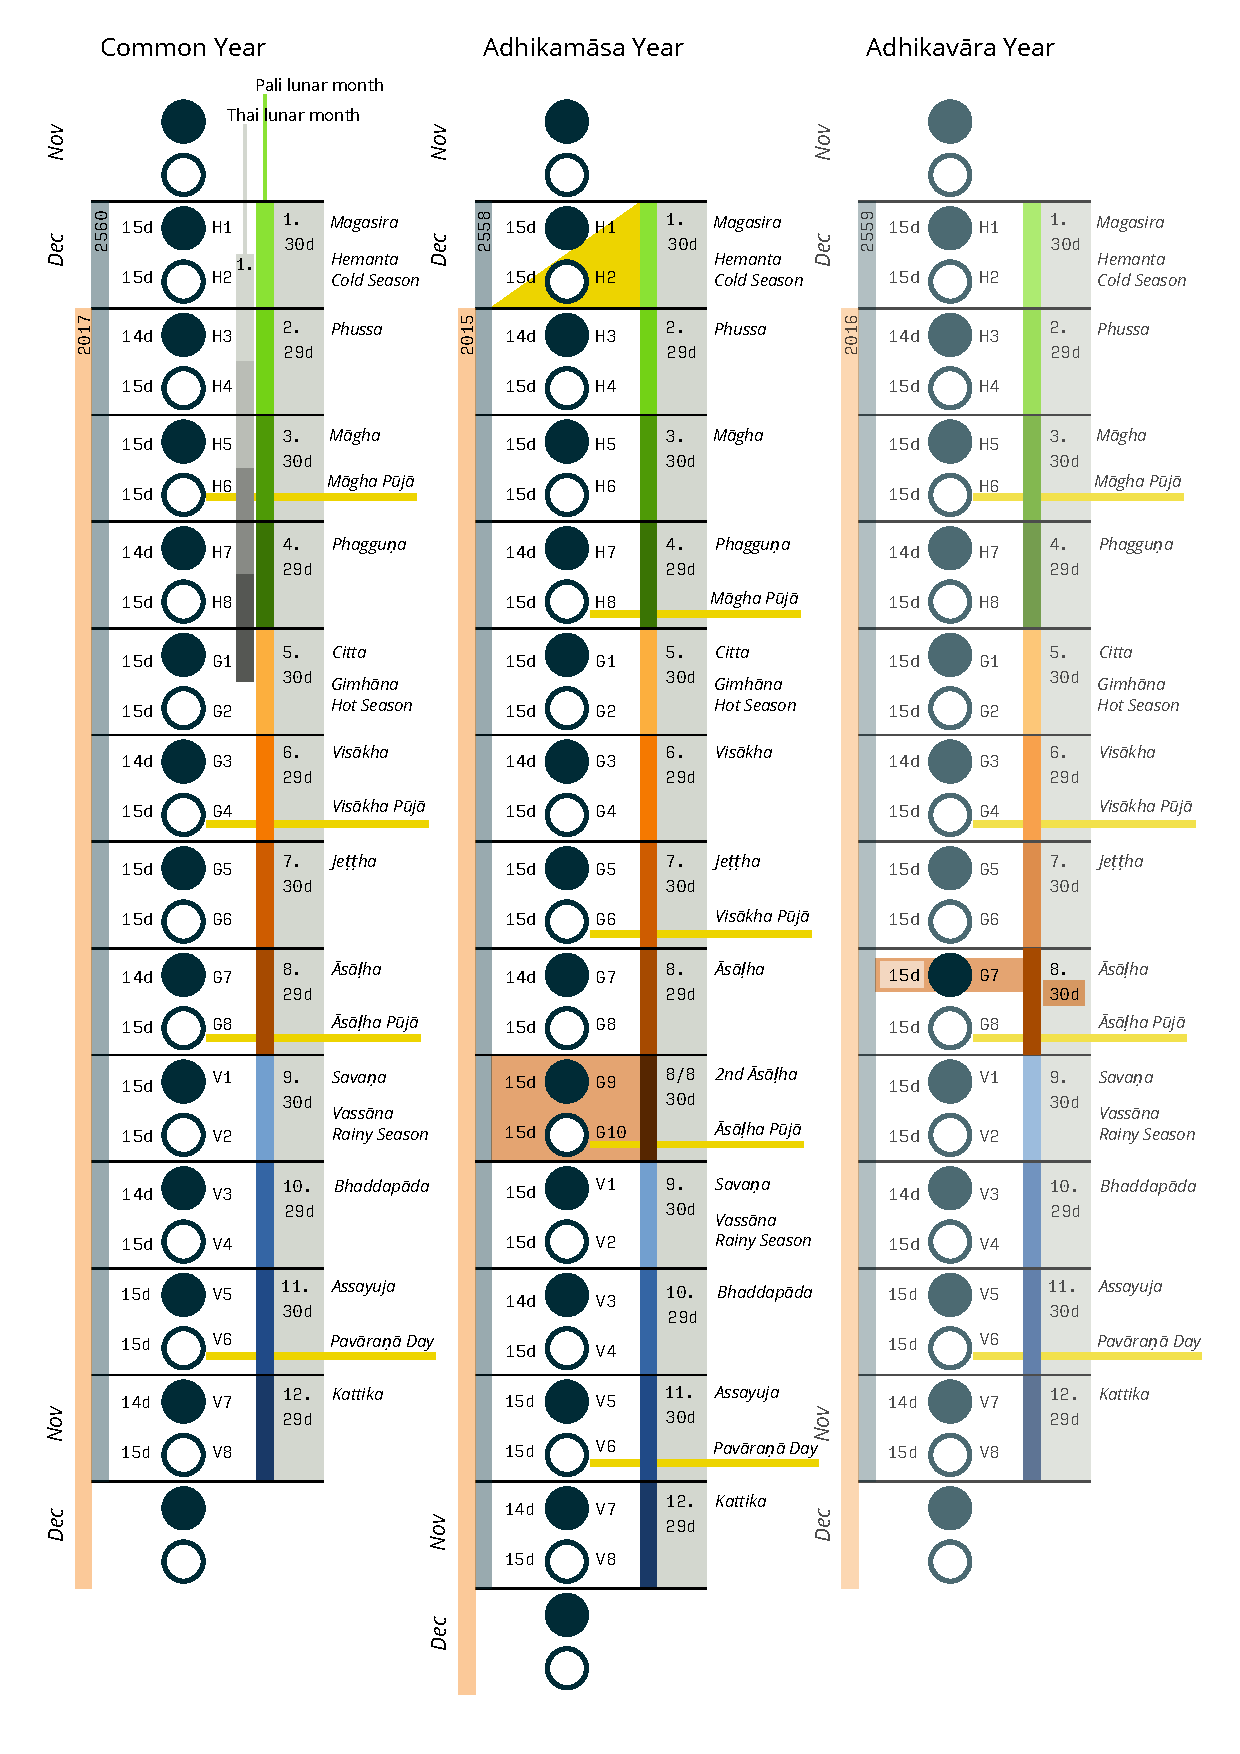
\includegraphics[width=\paperwidth]{common-adhikamasa-adhikavara.pdf}%
}

\fullpage{%
\label{year-2015}%
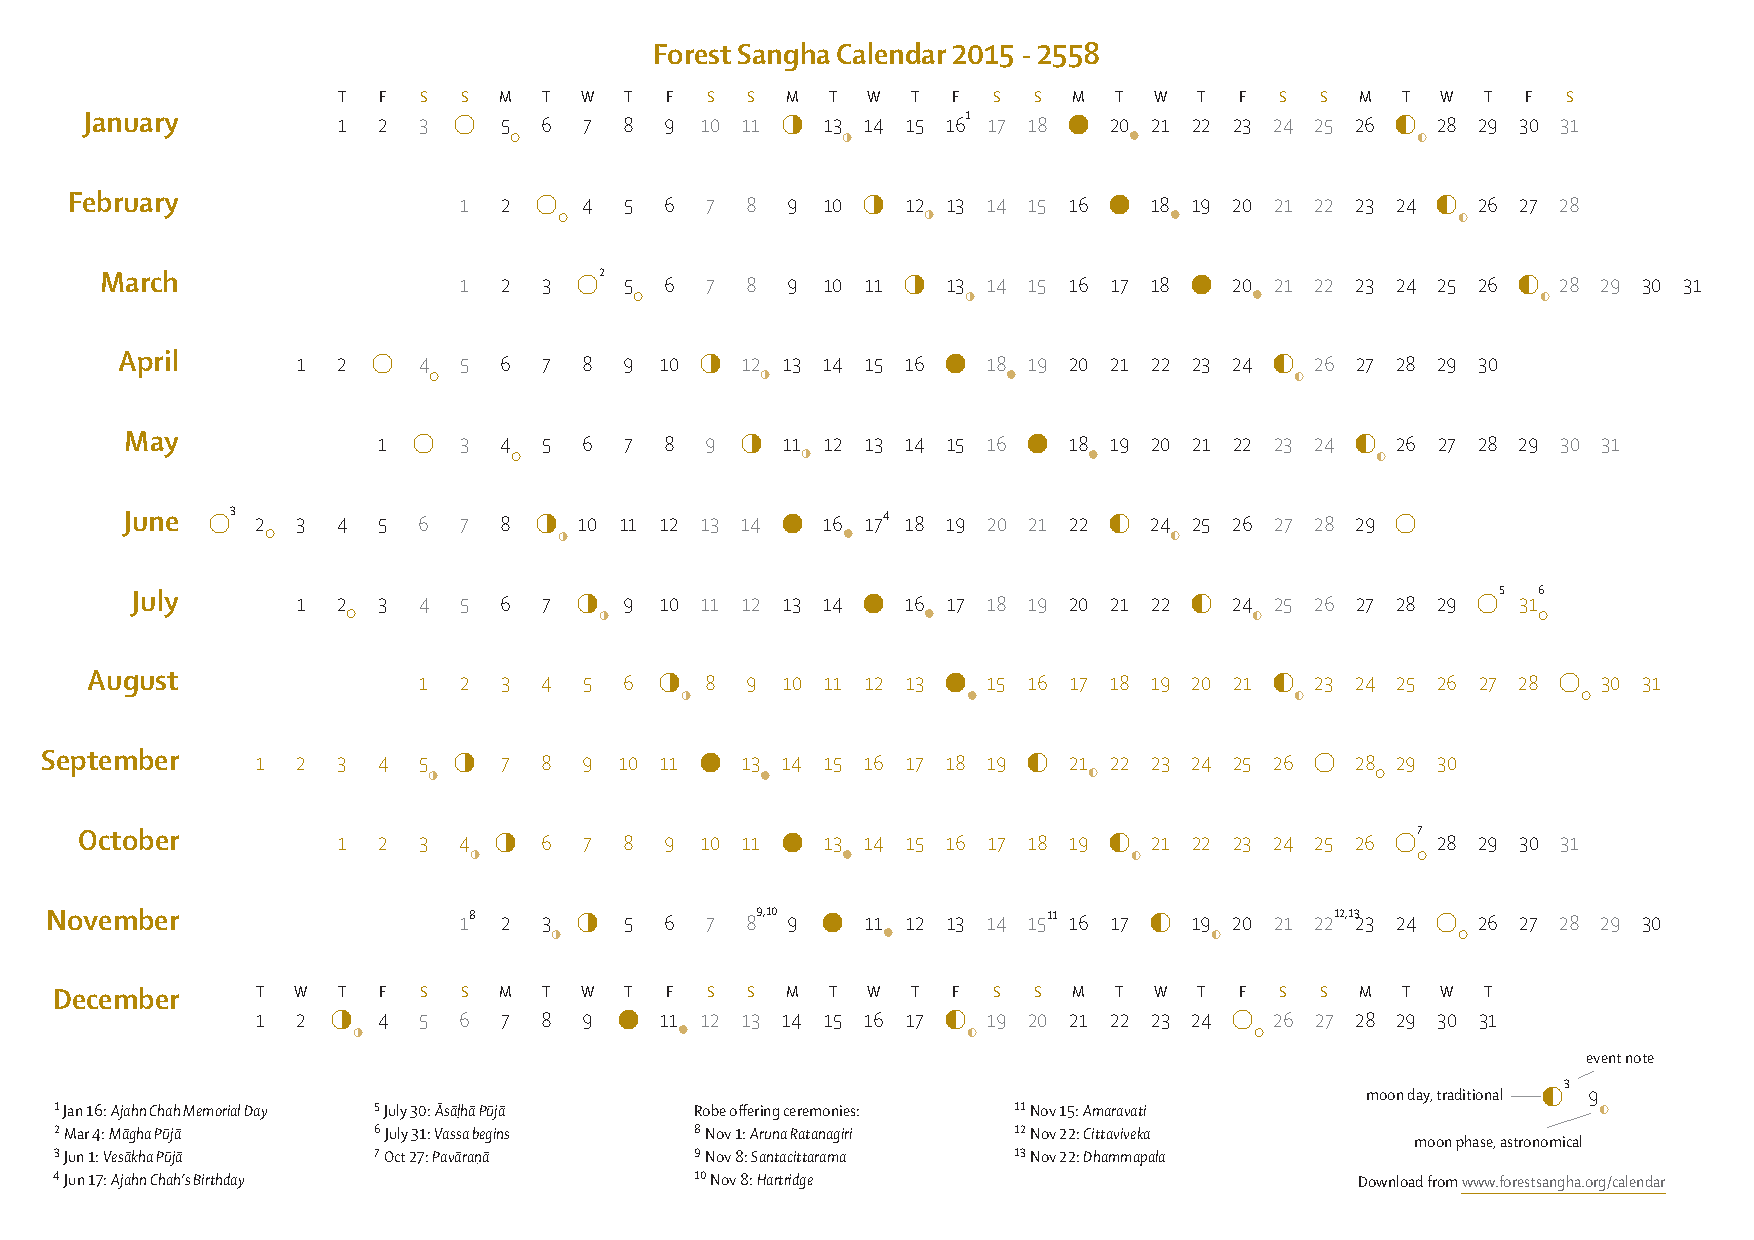
\includegraphics[angle=90,width=\paperwidth]{2015-fs-year-planner-A4.pdf}%
}

\fullpage{%
\label{year-2016}%
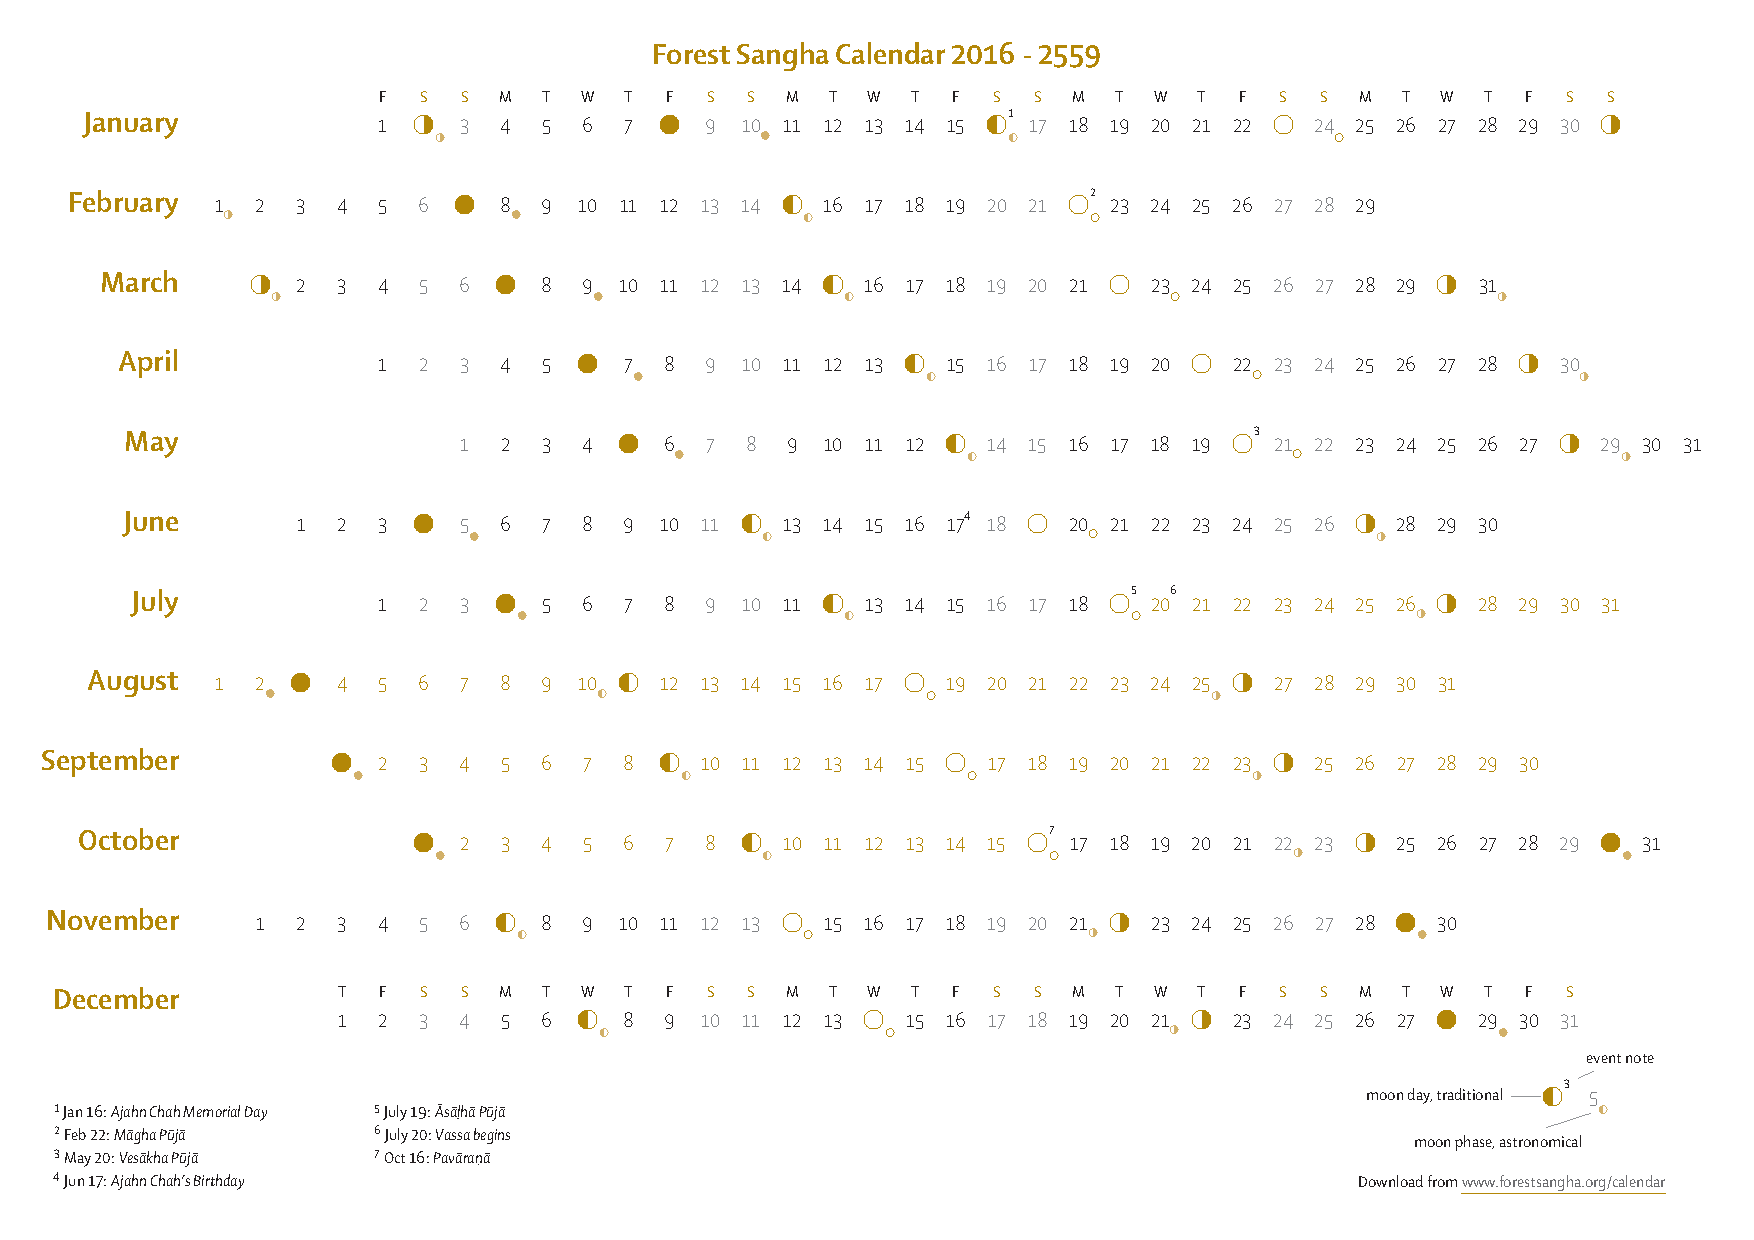
\includegraphics[angle=90,width=\paperwidth]{2016-fs-year-planner-A4.pdf}%
}

\fullpage{%
\label{year-2017}%
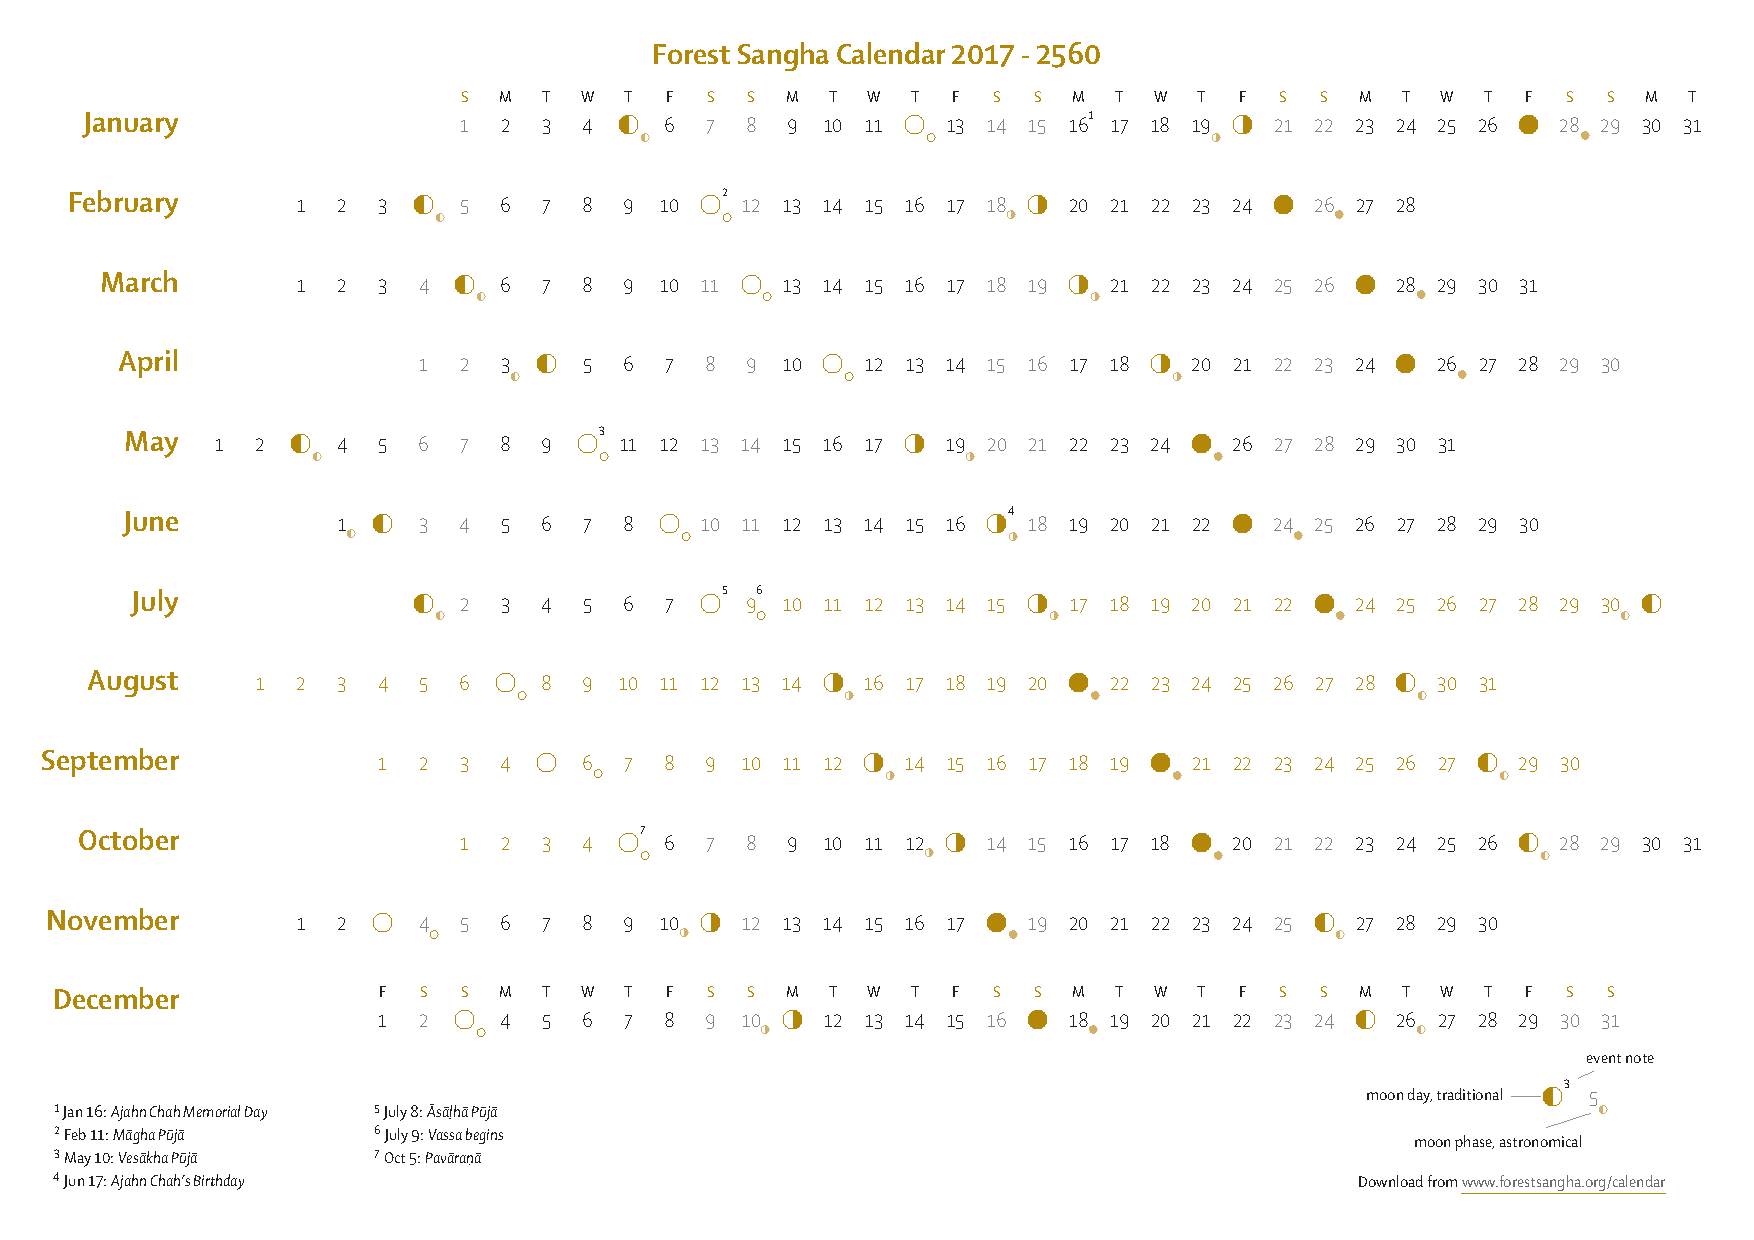
\includegraphics[angle=90,width=\paperwidth]{2017-fs-year-planner-A4.pdf}%
}
% Emacs 25.0.50.1 (Org mode 8.2.10)
\end{document}